\documentclass[1p]{elsarticle_modified}
%\bibliographystyle{elsarticle-num}

%\usepackage[colorlinks]{hyperref}
%\usepackage{abbrmath_seonhwa} %\Abb, \Ascr, \Acal ,\Abf, \Afrak
\usepackage{amsfonts}
\usepackage{amssymb}
\usepackage{amsmath}
\usepackage{amsthm}
\usepackage{scalefnt}
\usepackage{amsbsy}
\usepackage{kotex}
\usepackage{caption}
\usepackage{subfig}
\usepackage{color}
\usepackage{graphicx}
\usepackage{xcolor} %% white, black, red, green, blue, cyan, magenta, yellow
\usepackage{float}
\usepackage{setspace}
\usepackage{hyperref}

\usepackage{tikz}
\usetikzlibrary{arrows}

\usepackage{multirow}
\usepackage{array} % fixed length table
\usepackage{hhline}

%%%%%%%%%%%%%%%%%%%%%
\makeatletter
\renewcommand*\env@matrix[1][\arraystretch]{%
	\edef\arraystretch{#1}%
	\hskip -\arraycolsep
	\let\@ifnextchar\new@ifnextchar
	\array{*\c@MaxMatrixCols c}}
\makeatother %https://tex.stackexchange.com/questions/14071/how-can-i-increase-the-line-spacing-in-a-matrix
%%%%%%%%%%%%%%%

\usepackage[normalem]{ulem}

\newcommand{\msout}[1]{\ifmmode\text{\sout{\ensuremath{#1}}}\else\sout{#1}\fi}
%SOURCE: \msout is \stkout macro in https://tex.stackexchange.com/questions/20609/strikeout-in-math-mode

\newcommand{\cancel}[1]{
	\ifmmode
	{\color{red}\msout{#1}}
	\else
	{\color{red}\sout{#1}}
	\fi
}

\newcommand{\add}[1]{
	{\color{blue}\uwave{#1}}
}

\newcommand{\replace}[2]{
	\ifmmode
	{\color{red}\msout{#1}}{\color{blue}\uwave{#2}}
	\else
	{\color{red}\sout{#1}}{\color{blue}\uwave{#2}}
	\fi
}

\newcommand{\Sol}{\mathcal{S}} %segment
\newcommand{\D}{D} %diagram
\newcommand{\A}{\mathcal{A}} %arc


%%%%%%%%%%%%%%%%%%%%%%%%%%%%%5 test

\def\sl{\operatorname{\textup{SL}}(2,\Cbb)}
\def\psl{\operatorname{\textup{PSL}}(2,\Cbb)}
\def\quan{\mkern 1mu \triangleright \mkern 1mu}

\theoremstyle{definition}
\newtheorem{thm}{Theorem}[section]
\newtheorem{prop}[thm]{Proposition}
\newtheorem{lem}[thm]{Lemma}
\newtheorem{ques}[thm]{Question}
\newtheorem{cor}[thm]{Corollary}
\newtheorem{defn}[thm]{Definition}
\newtheorem{exam}[thm]{Example}
\newtheorem{rmk}[thm]{Remark}
\newtheorem{alg}[thm]{Algorithm}

\newcommand{\I}{\sqrt{-1}}
\begin{document}

%\begin{frontmatter}
%
%\title{Boundary parabolic representations of knots up to 8 crossings}
%
%%% Group authors per affiliation:
%\author{Yunhi Cho} 
%\address{Department of Mathematics, University of Seoul, Seoul, Korea}
%\ead{yhcho@uos.ac.kr}
%
%
%\author{Seonhwa Kim} %\fnref{s_kim}}
%\address{Center for Geometry and Physics, Institute for Basic Science, Pohang, 37673, Korea}
%\ead{ryeona17@ibs.re.kr}
%
%\author{Hyuk Kim}
%\address{Department of Mathematical Sciences, Seoul National University, Seoul 08826, Korea}
%\ead{hyukkim@snu.ac.kr}
%
%\author{Seokbeom Yoon}
%\address{Department of Mathematical Sciences, Seoul National University, Seoul, 08826,  Korea}
%\ead{sbyoon15@snu.ac.kr}
%
%\begin{abstract}
%We find all boundary parabolic representation of knots up to 8 crossings.
%
%\end{abstract}
%\begin{keyword}
%    \MSC[2010] 57M25 
%\end{keyword}
%
%\end{frontmatter}

%\linenumbers
%\tableofcontents
%
\newcommand\colored[1]{\textcolor{white}{\rule[-0.35ex]{0.8em}{1.4ex}}\kern-0.8em\color{red} #1}%
%\newcommand\colored[1]{\textcolor{white}{ #1}\kern-2.17ex	\textcolor{white}{ #1}\kern-1.81ex	\textcolor{white}{ #1}\kern-2.15ex\color{red}#1	}

{\Large $\underline{12a_{0846}~(K12a_{0846})}$}

\setlength{\tabcolsep}{10pt}
\renewcommand{\arraystretch}{1.6}
\vspace{1cm}\begin{tabular}{m{100pt}>{\centering\arraybackslash}m{274pt}}
\multirow{5}{120pt}{
	\centering
	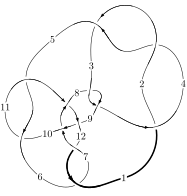
\includegraphics[width=112pt]{../../../GIT/diagram.site/Diagrams/png/1647_12a_0846.png}\\
\ \ \ A knot diagram\footnotemark}&
\allowdisplaybreaks
\textbf{Linearized knot diagam} \\
\cline{2-2}
 &
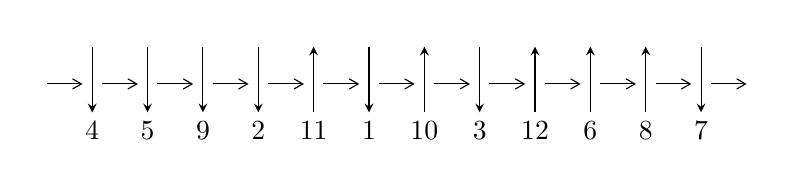
\begin{tikzpicture}[x=20pt, y=17pt]
	% nodes
	\node (C0) at (0, 0) {};
	\node (C1) at (1, 0) {};
	\node (C1U) at (1, +1) {};
	\node (C1D) at (1, -1) {4};

	\node (C2) at (2, 0) {};
	\node (C2U) at (2, +1) {};
	\node (C2D) at (2, -1) {5};

	\node (C3) at (3, 0) {};
	\node (C3U) at (3, +1) {};
	\node (C3D) at (3, -1) {9};

	\node (C4) at (4, 0) {};
	\node (C4U) at (4, +1) {};
	\node (C4D) at (4, -1) {2};

	\node (C5) at (5, 0) {};
	\node (C5U) at (5, +1) {};
	\node (C5D) at (5, -1) {11};

	\node (C6) at (6, 0) {};
	\node (C6U) at (6, +1) {};
	\node (C6D) at (6, -1) {1};

	\node (C7) at (7, 0) {};
	\node (C7U) at (7, +1) {};
	\node (C7D) at (7, -1) {10};

	\node (C8) at (8, 0) {};
	\node (C8U) at (8, +1) {};
	\node (C8D) at (8, -1) {3};

	\node (C9) at (9, 0) {};
	\node (C9U) at (9, +1) {};
	\node (C9D) at (9, -1) {12};

	\node (C10) at (10, 0) {};
	\node (C10U) at (10, +1) {};
	\node (C10D) at (10, -1) {6};

	\node (C11) at (11, 0) {};
	\node (C11U) at (11, +1) {};
	\node (C11D) at (11, -1) {8};

	\node (C12) at (12, 0) {};
	\node (C12U) at (12, +1) {};
	\node (C12D) at (12, -1) {7};
	\node (C13) at (13, 0) {};

	% arrows
	\draw[->,>={angle 60}]
	(C0) edge (C1) (C1) edge (C2) (C2) edge (C3) (C3) edge (C4) (C4) edge (C5) (C5) edge (C6) (C6) edge (C7) (C7) edge (C8) (C8) edge (C9) (C9) edge (C10) (C10) edge (C11) (C11) edge (C12) (C12) edge (C13) ;	\draw[->,>=stealth]
	(C1U) edge (C1D) (C2U) edge (C2D) (C3U) edge (C3D) (C4U) edge (C4D) (C5D) edge (C5U) (C6U) edge (C6D) (C7D) edge (C7U) (C8U) edge (C8D) (C9D) edge (C9U) (C10D) edge (C10U) (C11D) edge (C11U) (C12U) edge (C12D) ;
	\end{tikzpicture} \\
\hhline{~~} \\& 
\textbf{Solving Sequence} \\ \cline{2-2} 
 &
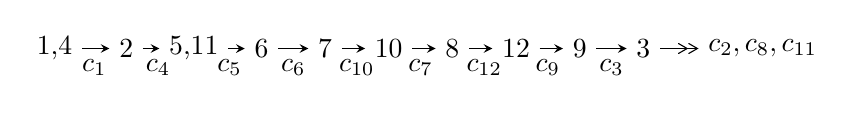
\begin{tikzpicture}[x=23pt, y=7pt]
	% node
	\node (A0) at (-1/8, 0) {1,4};
	\node (A1) at (1, 0) {2};
	\node (A2) at (33/16, 0) {5,11};
	\node (A3) at (25/8, 0) {6};
	\node (A4) at (33/8, 0) {7};
	\node (A5) at (41/8, 0) {10};
	\node (A6) at (49/8, 0) {8};
	\node (A7) at (57/8, 0) {12};
	\node (A8) at (65/8, 0) {9};
	\node (A9) at (73/8, 0) {3};
	\node (C1) at (1/2, -1) {$c_{1}$};
	\node (C2) at (3/2, -1) {$c_{4}$};
	\node (C3) at (21/8, -1) {$c_{5}$};
	\node (C4) at (29/8, -1) {$c_{6}$};
	\node (C5) at (37/8, -1) {$c_{10}$};
	\node (C6) at (45/8, -1) {$c_{7}$};
	\node (C7) at (53/8, -1) {$c_{12}$};
	\node (C8) at (61/8, -1) {$c_{9}$};
	\node (C9) at (69/8, -1) {$c_{3}$};
	\node (A10) at (11, 0) {$c_{2},c_{8},c_{11}$};

	% edge
	\draw[->,>=stealth]	
	(A0) edge (A1) (A1) edge (A2) (A2) edge (A3) (A3) edge (A4) (A4) edge (A5) (A5) edge (A6) (A6) edge (A7) (A7) edge (A8) (A8) edge (A9) ;
	\draw[->>,>={angle 60}]	
	(A9) edge (A10);
\end{tikzpicture} \\ 

\end{tabular} \\

\footnotetext{
The image of knot diagram is generated by the software ``\textbf{Draw programme}" developed by Andrew Bartholomew(\url{http://www.layer8.co.uk/maths/draw/index.htm\#Running-draw}), where we modified some parts for our purpose(\url{https://github.com/CATsTAILs/LinksPainter}).
}\phantom \\ \newline 
\centering \textbf{Ideals for irreducible components\footnotemark of $X_{\text{par}}$} 
 
\begin{align*}
I^u_{1}&=\langle 
-1.09278\times10^{260} u^{129}-1.32449\times10^{261} u^{128}+\cdots+3.80012\times10^{256} b+2.54286\times10^{261},\\
\phantom{I^u_{1}}&\phantom{= \langle  }5.57550\times10^{259} u^{129}+8.45930\times10^{260} u^{128}+\cdots+7.60023\times10^{256} a-5.21843\times10^{261},\\
\phantom{I^u_{1}}&\phantom{= \langle  }u^{130}+14 u^{129}+\cdots-35 u-49\rangle \\
I^u_{2}&=\langle 
5 u^{19}+12 u^{18}+\cdots+b+5,\;3 u^{19}+11 u^{18}+\cdots+a+11 u,\;u^{20}+4 u^{19}+\cdots-5 u+1\rangle \\
I^u_{3}&=\langle 
18445 a^8-60477 a^7+69483 a^6-21043 a^5-6071 a^4-11267 a^3+12888 a^2+1627 b-373 a-4047,\\
\phantom{I^u_{3}}&\phantom{= \langle  }7 a^9-20 a^8+16 a^7+5 a^6-7 a^5-6 a^4+4 a^3+3 a^2-2 a-1,\;u-1\rangle \\
\\
\end{align*}
\raggedright * 3 irreducible components of $\dim_{\mathbb{C}}=0$, with total 159 representations.\\
\footnotetext{All coefficients of polynomials are rational numbers. But the coefficients are sometimes approximated in decimal forms when there is not enough margin.}
\newpage
\renewcommand{\arraystretch}{1}
\centering \section*{I. $I^u_{1}= \langle -1.09\times10^{260} u^{129}-1.32\times10^{261} u^{128}+\cdots+3.80\times10^{256} b+2.54\times10^{261},\;5.58\times10^{259} u^{129}+8.46\times10^{260} u^{128}+\cdots+7.60\times10^{256} a-5.22\times10^{261},\;u^{130}+14 u^{129}+\cdots-35 u-49 \rangle$}
\flushleft \textbf{(i) Arc colorings}\\
\begin{tabular}{m{7pt} m{180pt} m{7pt} m{180pt} }
\flushright $a_{1}=$&$\begin{pmatrix}1\\0\end{pmatrix}$ \\
\flushright $a_{4}=$&$\begin{pmatrix}0\\u\end{pmatrix}$ \\
\flushright $a_{2}=$&$\begin{pmatrix}1\\u^2\end{pmatrix}$ \\
\flushright $a_{5}=$&$\begin{pmatrix}- u\\- u^3+u\end{pmatrix}$ \\
\flushright $a_{11}=$&$\begin{pmatrix}-733.595 u^{129}-11130.3 u^{128}+\cdots-27344.6 u+68661.4\\2875.66 u^{129}+34853.9 u^{128}+\cdots-23132.5 u-66915.3\end{pmatrix}$ \\
\flushright $a_{6}=$&$\begin{pmatrix}2327.78 u^{129}+29108.4 u^{128}+\cdots-4815.65 u-75259.4\\4875.30 u^{129}+60798.0 u^{128}+\cdots-13534.6 u-153050.\end{pmatrix}$ \\
\flushright $a_{7}=$&$\begin{pmatrix}-2547.52 u^{129}-31689.7 u^{128}+\cdots+8718.97 u+77790.6\\4875.30 u^{129}+60798.0 u^{128}+\cdots-13534.6 u-153050.\end{pmatrix}$ \\
\flushright $a_{10}=$&$\begin{pmatrix}2968.38 u^{129}+38020.6 u^{128}+\cdots+6385.70 u-116156.\\214.488 u^{129}+2233.99 u^{128}+\cdots-7504.88 u+3687.50\end{pmatrix}$ \\
\flushright $a_{8}=$&$\begin{pmatrix}-709.800 u^{129}-8902.49 u^{128}+\cdots+1399.03 u+23362.7\\1166.71 u^{129}+14805.6 u^{128}+\cdots+1012.59 u-42841.9\end{pmatrix}$ \\
\flushright $a_{12}=$&$\begin{pmatrix}-3174.46 u^{129}-40879.9 u^{128}+\cdots-10269.3 u+129353.\\2950.79 u^{129}+36205.8 u^{128}+\cdots-16869.5 u-79058.2\end{pmatrix}$ \\
\flushright $a_{9}=$&$\begin{pmatrix}681.193 u^{129}+8778.25 u^{128}+\cdots+3329.62 u-28655.4\\-2590.23 u^{129}-32855.2 u^{128}+\cdots-2287.68 u+95049.6\end{pmatrix}$ \\
\flushright $a_{3}=$&$\begin{pmatrix}- u^2+1\\- u^4+2 u^2\end{pmatrix}$\\&\end{tabular}
\flushleft \textbf{(ii) Obstruction class $= -1$}\\~\\
\flushleft \textbf{(iii) Cusp Shapes $= -5605.17 u^{129}-69784.3 u^{128}+\cdots+15066.8 u+174873.$}\\~\\
\newpage\renewcommand{\arraystretch}{1}
\flushleft \textbf{(iv) u-Polynomials at the component}\newline \\
\begin{tabular}{m{50pt}|m{274pt}}
Crossings & \hspace{64pt}u-Polynomials at each crossing \\
\hline $$\begin{aligned}c_{1},c_{2},c_{4}\end{aligned}$$&$\begin{aligned}
&u^{130}-14 u^{129}+\cdots+35 u-49
\end{aligned}$\\
\hline $$\begin{aligned}c_{3},c_{8}\end{aligned}$$&$\begin{aligned}
&u^{130}+u^{129}+\cdots-60928 u+25088
\end{aligned}$\\
\hline $$\begin{aligned}c_{5},c_{10}\end{aligned}$$&$\begin{aligned}
&u^{130}-2 u^{129}+\cdots-4232 u-4232
\end{aligned}$\\
\hline $$\begin{aligned}c_{6},c_{12}\end{aligned}$$&$\begin{aligned}
&u^{130}-3 u^{129}+\cdots+4534 u-71
\end{aligned}$\\
\hline $$\begin{aligned}c_{7}\end{aligned}$$&$\begin{aligned}
&u^{130}+10 u^{129}+\cdots-27 u-9
\end{aligned}$\\
\hline $$\begin{aligned}c_{9}\end{aligned}$$&$\begin{aligned}
&u^{130}+18 u^{129}+\cdots-8409 u+1079
\end{aligned}$\\
\hline $$\begin{aligned}c_{11}\end{aligned}$$&$\begin{aligned}
&u^{130}+u^{129}+\cdots-15153510 u-893777
\end{aligned}$\\
\hline
\end{tabular}\\~\\
\newpage\renewcommand{\arraystretch}{1}
\flushleft \textbf{(v) Riley Polynomials at the component}\newline \\
\begin{tabular}{m{50pt}|m{274pt}}
Crossings & \hspace{64pt}Riley Polynomials at each crossing \\
\hline $$\begin{aligned}c_{1},c_{2},c_{4}\end{aligned}$$&$\begin{aligned}
&y^{130}-122 y^{129}+\cdots-5929 y+2401
\end{aligned}$\\
\hline $$\begin{aligned}c_{3},c_{8}\end{aligned}$$&$\begin{aligned}
&y^{130}-69 y^{129}+\cdots-11984437248 y+629407744
\end{aligned}$\\
\hline $$\begin{aligned}c_{5},c_{10}\end{aligned}$$&$\begin{aligned}
&y^{130}+86 y^{129}+\cdots+519774240 y+17909824
\end{aligned}$\\
\hline $$\begin{aligned}c_{6},c_{12}\end{aligned}$$&$\begin{aligned}
&y^{130}+81 y^{129}+\cdots-16239788 y+5041
\end{aligned}$\\
\hline $$\begin{aligned}c_{7}\end{aligned}$$&$\begin{aligned}
&y^{130}-6 y^{129}+\cdots+2151 y+81
\end{aligned}$\\
\hline $$\begin{aligned}c_{9}\end{aligned}$$&$\begin{aligned}
&y^{130}-26 y^{129}+\cdots-102045441 y+1164241
\end{aligned}$\\
\hline $$\begin{aligned}c_{11}\end{aligned}$$&$\begin{aligned}
&y^{130}+13 y^{129}+\cdots+20581982318772 y+798837325729
\end{aligned}$\\
\hline
\end{tabular}\\~\\
\newpage\flushleft \textbf{(vi) Complex Volumes and Cusp Shapes}
$$\begin{array}{c|c|c}  
\text{Solutions to }I^u_{1}& \I (\text{vol} + \sqrt{-1}CS) & \text{Cusp shape}\\
 \hline 
\begin{aligned}
u &= \phantom{-}0.328537 + 0.951554 I \\
a &= \phantom{-}1.274030 - 0.038467 I \\
b &= -1.19741 + 1.89741 I\end{aligned}
 & -0.4865 - 14.3089 I & \phantom{-0.000000 } 0 \\ \hline\begin{aligned}
u &= \phantom{-}0.328537 - 0.951554 I \\
a &= \phantom{-}1.274030 + 0.038467 I \\
b &= -1.19741 - 1.89741 I\end{aligned}
 & -0.4865 + 14.3089 I & \phantom{-0.000000 } 0 \\ \hline\begin{aligned}
u &= \phantom{-}0.925732 + 0.424462 I \\
a &= -0.347303 - 1.192700 I \\
b &= \phantom{-}0.225774 + 0.575562 I\end{aligned}
 & \phantom{-}1.39635 + 3.23709 I & \phantom{-0.000000 } 0 \\ \hline\begin{aligned}
u &= \phantom{-}0.925732 - 0.424462 I \\
a &= -0.347303 + 1.192700 I \\
b &= \phantom{-}0.225774 - 0.575562 I\end{aligned}
 & \phantom{-}1.39635 - 3.23709 I & \phantom{-0.000000 } 0 \\ \hline\begin{aligned}
u &= \phantom{-}0.858665 + 0.587059 I \\
a &= \phantom{-}1.116190 + 0.421322 I \\
b &= -0.18571 + 1.68368 I\end{aligned}
 & -5.66140 + 2.87702 I & \phantom{-0.000000 } 0 \\ \hline\begin{aligned}
u &= \phantom{-}0.858665 - 0.587059 I \\
a &= \phantom{-}1.116190 - 0.421322 I \\
b &= -0.18571 - 1.68368 I\end{aligned}
 & -5.66140 - 2.87702 I & \phantom{-0.000000 } 0 \\ \hline\begin{aligned}
u &= \phantom{-}1.074370 + 0.067387 I \\
a &= \phantom{-}2.71351 + 0.00240 I \\
b &= \phantom{-}0.93774 + 1.10701 I\end{aligned}
 & -0.42547 + 2.53758 I & \phantom{-0.000000 } 0 \\ \hline\begin{aligned}
u &= \phantom{-}1.074370 - 0.067387 I \\
a &= \phantom{-}2.71351 - 0.00240 I \\
b &= \phantom{-}0.93774 - 1.10701 I\end{aligned}
 & -0.42547 - 2.53758 I & \phantom{-0.000000 } 0 \\ \hline\begin{aligned}
u &= \phantom{-}1.017690 + 0.363111 I \\
a &= \phantom{-}0.750109 + 0.218017 I \\
b &= -0.612129 - 0.557038 I\end{aligned}
 & -4.78176 - 1.13220 I & \phantom{-0.000000 } 0 \\ \hline\begin{aligned}
u &= \phantom{-}1.017690 - 0.363111 I \\
a &= \phantom{-}0.750109 - 0.218017 I \\
b &= -0.612129 + 0.557038 I\end{aligned}
 & -4.78176 + 1.13220 I & \phantom{-0.000000 } 0\\
 \hline 
 \end{array}$$\newpage$$\begin{array}{c|c|c}  
\text{Solutions to }I^u_{1}& \I (\text{vol} + \sqrt{-1}CS) & \text{Cusp shape}\\
 \hline 
\begin{aligned}
u &= \phantom{-}0.326397 + 0.853815 I \\
a &= -0.843130 + 0.307087 I \\
b &= \phantom{-}0.13566 - 1.88854 I\end{aligned}
 & -4.00841 - 7.89339 I & \phantom{-0.000000 } 0 \\ \hline\begin{aligned}
u &= \phantom{-}0.326397 - 0.853815 I \\
a &= -0.843130 - 0.307087 I \\
b &= \phantom{-}0.13566 + 1.88854 I\end{aligned}
 & -4.00841 + 7.89339 I & \phantom{-0.000000 } 0 \\ \hline\begin{aligned}
u &= \phantom{-}0.547123 + 0.943513 I \\
a &= -0.894553 + 0.625707 I \\
b &= \phantom{-}0.10167 - 2.32803 I\end{aligned}
 & -1.42660 - 2.83814 I & \phantom{-0.000000 } 0 \\ \hline\begin{aligned}
u &= \phantom{-}0.547123 - 0.943513 I \\
a &= -0.894553 - 0.625707 I \\
b &= \phantom{-}0.10167 + 2.32803 I\end{aligned}
 & -1.42660 + 2.83814 I & \phantom{-0.000000 } 0 \\ \hline\begin{aligned}
u &= -0.378985 + 0.820019 I \\
a &= -1.070330 - 0.449410 I \\
b &= \phantom{-}0.28653 + 1.41351 I\end{aligned}
 & \phantom{-}3.12587 - 4.37430 I & \phantom{-0.000000 } 0 \\ \hline\begin{aligned}
u &= -0.378985 - 0.820019 I \\
a &= -1.070330 + 0.449410 I \\
b &= \phantom{-}0.28653 - 1.41351 I\end{aligned}
 & \phantom{-}3.12587 + 4.37430 I & \phantom{-0.000000 } 0 \\ \hline\begin{aligned}
u &= \phantom{-}0.613683 + 0.661203 I \\
a &= \phantom{-}1.223980 + 0.253281 I \\
b &= -0.026339 + 1.164490 I\end{aligned}
 & -2.89630 + 0.85409 I & \phantom{-0.000000 } 0 \\ \hline\begin{aligned}
u &= \phantom{-}0.613683 - 0.661203 I \\
a &= \phantom{-}1.223980 - 0.253281 I \\
b &= -0.026339 - 1.164490 I\end{aligned}
 & -2.89630 - 0.85409 I & \phantom{-0.000000 } 0 \\ \hline\begin{aligned}
u &= \phantom{-}0.456890 + 0.755947 I \\
a &= -0.566371 - 0.319790 I \\
b &= \phantom{-}0.30403 - 1.47097 I\end{aligned}
 & -2.38061 - 5.66774 I & \phantom{-0.000000 } 0 \\ \hline\begin{aligned}
u &= \phantom{-}0.456890 - 0.755947 I \\
a &= -0.566371 + 0.319790 I \\
b &= \phantom{-}0.30403 + 1.47097 I\end{aligned}
 & -2.38061 + 5.66774 I & \phantom{-0.000000 } 0\\
 \hline 
 \end{array}$$\newpage$$\begin{array}{c|c|c}  
\text{Solutions to }I^u_{1}& \I (\text{vol} + \sqrt{-1}CS) & \text{Cusp shape}\\
 \hline 
\begin{aligned}
u &= \phantom{-}0.310871 + 1.087400 I \\
a &= \phantom{-}1.53844 - 0.09507 I \\
b &= -2.17790 + 1.71738 I\end{aligned}
 & -0.99196 - 4.71706 I & \phantom{-0.000000 } 0 \\ \hline\begin{aligned}
u &= \phantom{-}0.310871 - 1.087400 I \\
a &= \phantom{-}1.53844 + 0.09507 I \\
b &= -2.17790 - 1.71738 I\end{aligned}
 & -0.99196 + 4.71706 I & \phantom{-0.000000 } 0 \\ \hline\begin{aligned}
u &= \phantom{-}0.281124 + 0.804317 I \\
a &= -0.815269 + 0.700780 I \\
b &= \phantom{-}0.302176 - 0.112938 I\end{aligned}
 & \phantom{-}3.35673 - 7.72625 I & \phantom{-0.000000 } 0 \\ \hline\begin{aligned}
u &= \phantom{-}0.281124 - 0.804317 I \\
a &= -0.815269 - 0.700780 I \\
b &= \phantom{-}0.302176 + 0.112938 I\end{aligned}
 & \phantom{-}3.35673 + 7.72625 I & \phantom{-0.000000 } 0 \\ \hline\begin{aligned}
u &= -1.163870 + 0.069350 I \\
a &= -0.404045 + 0.135763 I \\
b &= -0.768918 - 0.712141 I\end{aligned}
 & \phantom{-}1.52846 + 7.35278 I & \phantom{-0.000000 } 0 \\ \hline\begin{aligned}
u &= -1.163870 - 0.069350 I \\
a &= -0.404045 - 0.135763 I \\
b &= -0.768918 + 0.712141 I\end{aligned}
 & \phantom{-}1.52846 - 7.35278 I & \phantom{-0.000000 } 0 \\ \hline\begin{aligned}
u &= \phantom{-}0.820783\phantom{ +0.000000I} \\
a &= \phantom{-}1.05160\phantom{ +0.000000I} \\
b &= \phantom{-}0.0364198\phantom{ +0.000000I}\end{aligned}
 & -1.15012\phantom{ +0.000000I} & \phantom{-0.000000 } 0 \\ \hline\begin{aligned}
u &= \phantom{-}0.967020 + 0.706799 I \\
a &= -0.876124 + 0.280697 I \\
b &= -0.88322 - 1.97107 I\end{aligned}
 & -2.38605 + 8.61930 I & \phantom{-0.000000 } 0 \\ \hline\begin{aligned}
u &= \phantom{-}0.967020 - 0.706799 I \\
a &= -0.876124 - 0.280697 I \\
b &= -0.88322 + 1.97107 I\end{aligned}
 & -2.38605 - 8.61930 I & \phantom{-0.000000 } 0 \\ \hline\begin{aligned}
u &= \phantom{-}1.164850 + 0.314678 I \\
a &= \phantom{-}0.726113 - 0.266537 I \\
b &= \phantom{-}0.492041 - 0.078387 I\end{aligned}
 & -0.131132 - 1.178100 I & \phantom{-0.000000 } 0\\
 \hline 
 \end{array}$$\newpage$$\begin{array}{c|c|c}  
\text{Solutions to }I^u_{1}& \I (\text{vol} + \sqrt{-1}CS) & \text{Cusp shape}\\
 \hline 
\begin{aligned}
u &= \phantom{-}1.164850 - 0.314678 I \\
a &= \phantom{-}0.726113 + 0.266537 I \\
b &= \phantom{-}0.492041 + 0.078387 I\end{aligned}
 & -0.131132 + 1.178100 I & \phantom{-0.000000 } 0 \\ \hline\begin{aligned}
u &= \phantom{-}0.391027 + 0.684289 I \\
a &= \phantom{-}0.461372 + 0.327658 I \\
b &= -0.370357 - 0.824880 I\end{aligned}
 & -0.63869 - 3.79000 I & \phantom{-0.000000 } 0 \\ \hline\begin{aligned}
u &= \phantom{-}0.391027 - 0.684289 I \\
a &= \phantom{-}0.461372 - 0.327658 I \\
b &= -0.370357 + 0.824880 I\end{aligned}
 & -0.63869 + 3.79000 I & \phantom{-0.000000 } 0 \\ \hline\begin{aligned}
u &= \phantom{-}0.079052 + 0.768633 I \\
a &= \phantom{-}0.00874662 + 0.00398131 I \\
b &= \phantom{-}0.544900 - 0.096774 I\end{aligned}
 & \phantom{-}3.19605 - 2.75030 I & \phantom{-0.000000 } 0 \\ \hline\begin{aligned}
u &= \phantom{-}0.079052 - 0.768633 I \\
a &= \phantom{-}0.00874662 - 0.00398131 I \\
b &= \phantom{-}0.544900 + 0.096774 I\end{aligned}
 & \phantom{-}3.19605 + 2.75030 I & \phantom{-0.000000 } 0 \\ \hline\begin{aligned}
u &= \phantom{-}1.190180 + 0.318430 I \\
a &= \phantom{-}0.674856 - 0.624355 I \\
b &= \phantom{-}0.456322 - 0.062958 I\end{aligned}
 & -0.169062 - 1.292200 I & \phantom{-0.000000 } 0 \\ \hline\begin{aligned}
u &= \phantom{-}1.190180 - 0.318430 I \\
a &= \phantom{-}0.674856 + 0.624355 I \\
b &= \phantom{-}0.456322 + 0.062958 I\end{aligned}
 & -0.169062 + 1.292200 I & \phantom{-0.000000 } 0 \\ \hline\begin{aligned}
u &= -1.243070 + 0.082316 I \\
a &= -0.477105 + 0.673366 I \\
b &= -0.918203 - 0.239906 I\end{aligned}
 & \phantom{-}1.95452 - 0.73217 I & \phantom{-0.000000 } 0 \\ \hline\begin{aligned}
u &= -1.243070 - 0.082316 I \\
a &= -0.477105 - 0.673366 I \\
b &= -0.918203 + 0.239906 I\end{aligned}
 & \phantom{-}1.95452 + 0.73217 I & \phantom{-0.000000 } 0 \\ \hline\begin{aligned}
u &= \phantom{-}0.108093 + 0.744850 I \\
a &= -0.125117 + 0.426426 I \\
b &= \phantom{-}0.625444 - 0.004175 I\end{aligned}
 & \phantom{-}3.14662 - 2.57828 I & \phantom{-0.000000 } 0\\
 \hline 
 \end{array}$$\newpage$$\begin{array}{c|c|c}  
\text{Solutions to }I^u_{1}& \I (\text{vol} + \sqrt{-1}CS) & \text{Cusp shape}\\
 \hline 
\begin{aligned}
u &= \phantom{-}0.108093 - 0.744850 I \\
a &= -0.125117 - 0.426426 I \\
b &= \phantom{-}0.625444 + 0.004175 I\end{aligned}
 & \phantom{-}3.14662 + 2.57828 I & \phantom{-0.000000 } 0 \\ \hline\begin{aligned}
u &= \phantom{-}1.252820 + 0.043823 I \\
a &= \phantom{-}1.08094 + 2.93788 I \\
b &= \phantom{-}0.467723 + 0.557245 I\end{aligned}
 & -5.23503 - 0.36072 I & \phantom{-0.000000 } 0 \\ \hline\begin{aligned}
u &= \phantom{-}1.252820 - 0.043823 I \\
a &= \phantom{-}1.08094 - 2.93788 I \\
b &= \phantom{-}0.467723 - 0.557245 I\end{aligned}
 & -5.23503 + 0.36072 I & \phantom{-0.000000 } 0 \\ \hline\begin{aligned}
u &= \phantom{-}1.252870 + 0.067833 I \\
a &= \phantom{-}0.64482 - 4.73420 I \\
b &= \phantom{-}1.04580 - 1.78608 I\end{aligned}
 & -1.20363 - 3.45389 I & \phantom{-0.000000 } 0 \\ \hline\begin{aligned}
u &= \phantom{-}1.252870 - 0.067833 I \\
a &= \phantom{-}0.64482 + 4.73420 I \\
b &= \phantom{-}1.04580 + 1.78608 I\end{aligned}
 & -1.20363 + 3.45389 I & \phantom{-0.000000 } 0 \\ \hline\begin{aligned}
u &= -0.442581 + 0.598153 I \\
a &= \phantom{-}1.078450 - 0.503730 I \\
b &= -0.75287 - 1.55009 I\end{aligned}
 & \phantom{-}2.56590 + 8.61563 I & \phantom{-0.000000 } 0 \\ \hline\begin{aligned}
u &= -0.442581 - 0.598153 I \\
a &= \phantom{-}1.078450 + 0.503730 I \\
b &= -0.75287 + 1.55009 I\end{aligned}
 & \phantom{-}2.56590 - 8.61563 I & \phantom{-0.000000 } 0 \\ \hline\begin{aligned}
u &= \phantom{-}0.343983 + 0.636102 I \\
a &= \phantom{-}0.676314 + 0.731561 I \\
b &= \phantom{-}0.226933 + 0.763022 I\end{aligned}
 & -2.96488 - 2.11966 I & \phantom{-0.000000 } 0 \\ \hline\begin{aligned}
u &= \phantom{-}0.343983 - 0.636102 I \\
a &= \phantom{-}0.676314 - 0.731561 I \\
b &= \phantom{-}0.226933 - 0.763022 I\end{aligned}
 & -2.96488 + 2.11966 I & \phantom{-0.000000 } 0 \\ \hline\begin{aligned}
u &= -1.278240 + 0.076549 I \\
a &= \phantom{-}0.688761 - 0.362001 I \\
b &= \phantom{-}0.635930 - 0.936669 I\end{aligned}
 & -4.78653 - 1.59407 I & \phantom{-0.000000 } 0\\
 \hline 
 \end{array}$$\newpage$$\begin{array}{c|c|c}  
\text{Solutions to }I^u_{1}& \I (\text{vol} + \sqrt{-1}CS) & \text{Cusp shape}\\
 \hline 
\begin{aligned}
u &= -1.278240 - 0.076549 I \\
a &= \phantom{-}0.688761 + 0.362001 I \\
b &= \phantom{-}0.635930 + 0.936669 I\end{aligned}
 & -4.78653 + 1.59407 I & \phantom{-0.000000 } 0 \\ \hline\begin{aligned}
u &= \phantom{-}0.310436 + 0.645987 I \\
a &= -1.89400 - 0.01713 I \\
b &= \phantom{-}1.33565 - 1.76018 I\end{aligned}
 & \phantom{-}1.16491 - 5.17903 I & \phantom{-0.000000 } 0 \\ \hline\begin{aligned}
u &= \phantom{-}0.310436 - 0.645987 I \\
a &= -1.89400 + 0.01713 I \\
b &= \phantom{-}1.33565 + 1.76018 I\end{aligned}
 & \phantom{-}1.16491 + 5.17903 I & \phantom{-0.000000 } 0 \\ \hline\begin{aligned}
u &= \phantom{-}0.546564 + 0.459359 I \\
a &= \phantom{-}1.066240 + 0.221282 I \\
b &= -0.289619 + 0.130137 I\end{aligned}
 & -1.385150 - 0.269456 I & \phantom{-0.000000 } 0 \\ \hline\begin{aligned}
u &= \phantom{-}0.546564 - 0.459359 I \\
a &= \phantom{-}1.066240 - 0.221282 I \\
b &= -0.289619 - 0.130137 I\end{aligned}
 & -1.385150 + 0.269456 I & \phantom{-0.000000 } 0 \\ \hline\begin{aligned}
u &= \phantom{-}1.315590 + 0.071467 I \\
a &= -0.112675 - 0.790590 I \\
b &= -0.398404 - 0.494567 I\end{aligned}
 & -2.97910 - 1.77302 I & \phantom{-0.000000 } 0 \\ \hline\begin{aligned}
u &= \phantom{-}1.315590 - 0.071467 I \\
a &= -0.112675 + 0.790590 I \\
b &= -0.398404 + 0.494567 I\end{aligned}
 & -2.97910 + 1.77302 I & \phantom{-0.000000 } 0 \\ \hline\begin{aligned}
u &= \phantom{-}0.987474 + 0.878597 I \\
a &= \phantom{-}0.894909 - 0.344556 I \\
b &= \phantom{-}0.32266 + 2.47963 I\end{aligned}
 & -2.45297 - 3.70553 I & \phantom{-0.000000 } 0 \\ \hline\begin{aligned}
u &= \phantom{-}0.987474 - 0.878597 I \\
a &= \phantom{-}0.894909 + 0.344556 I \\
b &= \phantom{-}0.32266 - 2.47963 I\end{aligned}
 & -2.45297 + 3.70553 I & \phantom{-0.000000 } 0 \\ \hline\begin{aligned}
u &= \phantom{-}1.326740 + 0.196563 I \\
a &= -0.613407 + 0.123183 I \\
b &= \phantom{-}0.363905 - 0.317078 I\end{aligned}
 & \phantom{-}0.47369 - 5.68832 I & \phantom{-0.000000 } 0\\
 \hline 
 \end{array}$$\newpage$$\begin{array}{c|c|c}  
\text{Solutions to }I^u_{1}& \I (\text{vol} + \sqrt{-1}CS) & \text{Cusp shape}\\
 \hline 
\begin{aligned}
u &= \phantom{-}1.326740 - 0.196563 I \\
a &= -0.613407 - 0.123183 I \\
b &= \phantom{-}0.363905 + 0.317078 I\end{aligned}
 & \phantom{-}0.47369 + 5.68832 I & \phantom{-0.000000 } 0 \\ \hline\begin{aligned}
u &= -1.35728\phantom{ +0.000000I} \\
a &= \phantom{-}1.14882\phantom{ +0.000000I} \\
b &= \phantom{-}1.52745\phantom{ +0.000000I}\end{aligned}
 & -2.56238\phantom{ +0.000000I} & \phantom{-0.000000 } 0 \\ \hline\begin{aligned}
u &= -1.317810 + 0.326766 I \\
a &= \phantom{-}0.479988 + 0.466680 I \\
b &= \phantom{-}0.628510 + 0.171659 I\end{aligned}
 & -1.18088 + 6.70646 I & \phantom{-0.000000 } 0 \\ \hline\begin{aligned}
u &= -1.317810 - 0.326766 I \\
a &= \phantom{-}0.479988 - 0.466680 I \\
b &= \phantom{-}0.628510 - 0.171659 I\end{aligned}
 & -1.18088 - 6.70646 I & \phantom{-0.000000 } 0 \\ \hline\begin{aligned}
u &= \phantom{-}0.366768 + 0.520839 I \\
a &= -2.23423 - 1.57920 I \\
b &= \phantom{-}0.801086 - 0.369711 I\end{aligned}
 & -3.37537 - 1.30670 I & \phantom{-0.000000 } 0 \\ \hline\begin{aligned}
u &= \phantom{-}0.366768 - 0.520839 I \\
a &= -2.23423 + 1.57920 I \\
b &= \phantom{-}0.801086 + 0.369711 I\end{aligned}
 & -3.37537 + 1.30670 I & \phantom{-0.000000 } 0 \\ \hline\begin{aligned}
u &= \phantom{-}0.406976 + 0.459261 I \\
a &= \phantom{-}0.631498 - 0.737431 I \\
b &= \phantom{-}0.67086 + 1.79575 I\end{aligned}
 & \phantom{-}0.47179 + 1.76850 I & \phantom{-0.000000 } 0 \\ \hline\begin{aligned}
u &= \phantom{-}0.406976 - 0.459261 I \\
a &= \phantom{-}0.631498 + 0.737431 I \\
b &= \phantom{-}0.67086 - 1.79575 I\end{aligned}
 & \phantom{-}0.47179 - 1.76850 I & \phantom{-0.000000 } 0 \\ \hline\begin{aligned}
u &= -1.377590 + 0.183136 I \\
a &= \phantom{-}1.034860 + 0.508253 I \\
b &= \phantom{-}1.76292 - 0.74576 I\end{aligned}
 & -3.08113 + 0.81431 I & \phantom{-0.000000 } 0 \\ \hline\begin{aligned}
u &= -1.377590 - 0.183136 I \\
a &= \phantom{-}1.034860 - 0.508253 I \\
b &= \phantom{-}1.76292 + 0.74576 I\end{aligned}
 & -3.08113 - 0.81431 I & \phantom{-0.000000 } 0\\
 \hline 
 \end{array}$$\newpage$$\begin{array}{c|c|c}  
\text{Solutions to }I^u_{1}& \I (\text{vol} + \sqrt{-1}CS) & \text{Cusp shape}\\
 \hline 
\begin{aligned}
u &= -1.361960 + 0.297233 I \\
a &= \phantom{-}0.612441 - 0.128457 I \\
b &= \phantom{-}0.825978 - 0.180047 I\end{aligned}
 & -1.53269 + 6.33362 I & \phantom{-0.000000 } 0 \\ \hline\begin{aligned}
u &= -1.361960 - 0.297233 I \\
a &= \phantom{-}0.612441 + 0.128457 I \\
b &= \phantom{-}0.825978 + 0.180047 I\end{aligned}
 & -1.53269 - 6.33362 I & \phantom{-0.000000 } 0 \\ \hline\begin{aligned}
u &= \phantom{-}1.395060 + 0.057125 I \\
a &= \phantom{-}0.21679 - 2.46918 I \\
b &= \phantom{-}0.109256 - 1.376090 I\end{aligned}
 & -4.71583 - 3.31857 I & \phantom{-0.000000 } 0 \\ \hline\begin{aligned}
u &= \phantom{-}1.395060 - 0.057125 I \\
a &= \phantom{-}0.21679 + 2.46918 I \\
b &= \phantom{-}0.109256 + 1.376090 I\end{aligned}
 & -4.71583 + 3.31857 I & \phantom{-0.000000 } 0 \\ \hline\begin{aligned}
u &= \phantom{-}1.395630 + 0.187546 I \\
a &= -1.21124 - 2.32835 I \\
b &= -0.04024 - 1.84969 I\end{aligned}
 & -6.87980 - 5.59995 I & \phantom{-0.000000 } 0 \\ \hline\begin{aligned}
u &= \phantom{-}1.395630 - 0.187546 I \\
a &= -1.21124 + 2.32835 I \\
b &= -0.04024 + 1.84969 I\end{aligned}
 & -6.87980 + 5.59995 I & \phantom{-0.000000 } 0 \\ \hline\begin{aligned}
u &= -0.130721 + 0.564242 I \\
a &= -0.81966 - 1.40814 I \\
b &= -0.174294 + 0.402763 I\end{aligned}
 & \phantom{-}5.03065 + 2.91197 I & \phantom{-0.000000 } 0 \\ \hline\begin{aligned}
u &= -0.130721 - 0.564242 I \\
a &= -0.81966 + 1.40814 I \\
b &= -0.174294 - 0.402763 I\end{aligned}
 & \phantom{-}5.03065 - 2.91197 I & \phantom{-0.000000 } 0 \\ \hline\begin{aligned}
u &= -0.476447 + 0.316086 I \\
a &= \phantom{-}0.493099 - 0.642060 I \\
b &= -0.731484 - 1.186380 I\end{aligned}
 & \phantom{-}3.62319 - 0.56871 I & \phantom{-0.000000 } 0 \\ \hline\begin{aligned}
u &= -0.476447 - 0.316086 I \\
a &= \phantom{-}0.493099 + 0.642060 I \\
b &= -0.731484 + 1.186380 I\end{aligned}
 & \phantom{-}3.62319 + 0.56871 I & \phantom{-0.000000 } 0\\
 \hline 
 \end{array}$$\newpage$$\begin{array}{c|c|c}  
\text{Solutions to }I^u_{1}& \I (\text{vol} + \sqrt{-1}CS) & \text{Cusp shape}\\
 \hline 
\begin{aligned}
u &= -1.43415 + 0.18496 I \\
a &= \phantom{-}1.53348 - 2.15932 I \\
b &= \phantom{-}0.47839 - 2.33301 I\end{aligned}
 & -5.39383 + 0.67456 I & \phantom{-0.000000 } 0 \\ \hline\begin{aligned}
u &= -1.43415 - 0.18496 I \\
a &= \phantom{-}1.53348 + 2.15932 I \\
b &= \phantom{-}0.47839 + 2.33301 I\end{aligned}
 & -5.39383 - 0.67456 I & \phantom{-0.000000 } 0 \\ \hline\begin{aligned}
u &= -1.44236 + 0.10379 I \\
a &= \phantom{-}0.263305 - 0.348512 I \\
b &= \phantom{-}1.089260 - 0.781730 I\end{aligned}
 & -5.37237 - 2.41269 I & \phantom{-0.000000 } 0 \\ \hline\begin{aligned}
u &= -1.44236 - 0.10379 I \\
a &= \phantom{-}0.263305 + 0.348512 I \\
b &= \phantom{-}1.089260 + 0.781730 I\end{aligned}
 & -5.37237 + 2.41269 I & \phantom{-0.000000 } 0 \\ \hline\begin{aligned}
u &= -1.42708 + 0.25184 I \\
a &= -0.34989 + 2.76349 I \\
b &= \phantom{-}1.61491 + 2.06056 I\end{aligned}
 & -4.41116 + 8.47604 I & \phantom{-0.000000 } 0 \\ \hline\begin{aligned}
u &= -1.42708 - 0.25184 I \\
a &= -0.34989 - 2.76349 I \\
b &= \phantom{-}1.61491 - 2.06056 I\end{aligned}
 & -4.41116 - 8.47604 I & \phantom{-0.000000 } 0 \\ \hline\begin{aligned}
u &= -1.43628 + 0.20856 I \\
a &= -0.22358 + 1.73503 I \\
b &= \phantom{-}1.196200 + 0.638607 I\end{aligned}
 & -9.16387 + 4.05703 I & \phantom{-0.000000 } 0 \\ \hline\begin{aligned}
u &= -1.43628 - 0.20856 I \\
a &= -0.22358 - 1.73503 I \\
b &= \phantom{-}1.196200 - 0.638607 I\end{aligned}
 & -9.16387 - 4.05703 I & \phantom{-0.000000 } 0 \\ \hline\begin{aligned}
u &= -1.44630 + 0.17990 I \\
a &= -0.165006 - 0.086158 I \\
b &= -0.853185 + 0.249209 I\end{aligned}
 & -7.57713 + 2.60992 I & \phantom{-0.000000 } 0 \\ \hline\begin{aligned}
u &= -1.44630 - 0.17990 I \\
a &= -0.165006 + 0.086158 I \\
b &= -0.853185 - 0.249209 I\end{aligned}
 & -7.57713 - 2.60992 I & \phantom{-0.000000 } 0\\
 \hline 
 \end{array}$$\newpage$$\begin{array}{c|c|c}  
\text{Solutions to }I^u_{1}& \I (\text{vol} + \sqrt{-1}CS) & \text{Cusp shape}\\
 \hline 
\begin{aligned}
u &= -1.44080 + 0.23751 I \\
a &= \phantom{-}0.97728 - 1.53055 I \\
b &= \phantom{-}0.233743 - 1.166650 I\end{aligned}
 & -8.72321 + 5.31358 I & \phantom{-0.000000 } 0 \\ \hline\begin{aligned}
u &= -1.44080 - 0.23751 I \\
a &= \phantom{-}0.97728 + 1.53055 I \\
b &= \phantom{-}0.233743 + 1.166650 I\end{aligned}
 & -8.72321 - 5.31358 I & \phantom{-0.000000 } 0 \\ \hline\begin{aligned}
u &= -1.43345 + 0.31707 I \\
a &= -0.146080 - 0.442910 I \\
b &= \phantom{-}0.451725 - 0.171945 I\end{aligned}
 & -2.13477 + 11.78310 I & \phantom{-0.000000 } 0 \\ \hline\begin{aligned}
u &= -1.43345 - 0.31707 I \\
a &= -0.146080 + 0.442910 I \\
b &= \phantom{-}0.451725 + 0.171945 I\end{aligned}
 & -2.13477 - 11.78310 I & \phantom{-0.000000 } 0 \\ \hline\begin{aligned}
u &= -1.45299 + 0.24669 I \\
a &= -0.670793 + 0.589860 I \\
b &= -0.83242 + 1.14754 I\end{aligned}
 & -6.57708 + 7.15153 I & \phantom{-0.000000 } 0 \\ \hline\begin{aligned}
u &= -1.45299 - 0.24669 I \\
a &= -0.670793 - 0.589860 I \\
b &= -0.83242 - 1.14754 I\end{aligned}
 & -6.57708 - 7.15153 I & \phantom{-0.000000 } 0 \\ \hline\begin{aligned}
u &= -0.220048 + 0.470245 I \\
a &= -1.45606 + 0.27415 I \\
b &= \phantom{-}0.132066 + 1.362320 I\end{aligned}
 & -1.67452 + 3.13091 I & \phantom{-0.000000 } 0. - 4.61042 I \\ \hline\begin{aligned}
u &= -0.220048 - 0.470245 I \\
a &= -1.45606 - 0.27415 I \\
b &= \phantom{-}0.132066 - 1.362320 I\end{aligned}
 & -1.67452 - 3.13091 I & \phantom{-0.000000 -}0. + 4.61042 I \\ \hline\begin{aligned}
u &= \phantom{-}0.169375 + 0.489161 I \\
a &= -2.69024 - 0.96416 I \\
b &= \phantom{-}1.33643 + 1.10743 I\end{aligned}
 & \phantom{-}1.88655 + 1.65023 I & \phantom{-0.000000 } 0 \\ \hline\begin{aligned}
u &= \phantom{-}0.169375 - 0.489161 I \\
a &= -2.69024 + 0.96416 I \\
b &= \phantom{-}1.33643 - 1.10743 I\end{aligned}
 & \phantom{-}1.88655 - 1.65023 I & \phantom{-0.000000 } 0\\
 \hline 
 \end{array}$$\newpage$$\begin{array}{c|c|c}  
\text{Solutions to }I^u_{1}& \I (\text{vol} + \sqrt{-1}CS) & \text{Cusp shape}\\
 \hline 
\begin{aligned}
u &= \phantom{-}1.46709 + 0.23777 I \\
a &= \phantom{-}0.37141 + 2.44450 I \\
b &= -1.06288 + 1.98251 I\end{aligned}
 & -3.56917 - 11.75340 I & \phantom{-0.000000 } 0 \\ \hline\begin{aligned}
u &= \phantom{-}1.46709 - 0.23777 I \\
a &= \phantom{-}0.37141 - 2.44450 I \\
b &= -1.06288 - 1.98251 I\end{aligned}
 & -3.56917 + 11.75340 I & \phantom{-0.000000 } 0 \\ \hline\begin{aligned}
u &= -1.45682 + 0.33683 I \\
a &= -1.25834 + 1.75821 I \\
b &= \phantom{-}0.29126 + 2.12439 I\end{aligned}
 & -9.7181 + 12.1998 I & \phantom{-0.000000 } 0 \\ \hline\begin{aligned}
u &= -1.45682 - 0.33683 I \\
a &= -1.25834 - 1.75821 I \\
b &= \phantom{-}0.29126 - 2.12439 I\end{aligned}
 & -9.7181 - 12.1998 I & \phantom{-0.000000 } 0 \\ \hline\begin{aligned}
u &= -1.49467 + 0.27154 I \\
a &= -0.60073 + 1.97944 I \\
b &= \phantom{-}0.42932 + 1.82551 I\end{aligned}
 & -8.70050 + 9.40227 I & \phantom{-0.000000 } 0 \\ \hline\begin{aligned}
u &= -1.49467 - 0.27154 I \\
a &= -0.60073 - 1.97944 I \\
b &= \phantom{-}0.42932 - 1.82551 I\end{aligned}
 & -8.70050 - 9.40227 I & \phantom{-0.000000 } 0 \\ \hline\begin{aligned}
u &= -1.47646 + 0.38036 I \\
a &= \phantom{-}0.69606 - 2.10476 I \\
b &= -1.44135 - 1.94162 I\end{aligned}
 & -6.2538 + 19.1081 I & \phantom{-0.000000 } 0 \\ \hline\begin{aligned}
u &= -1.47646 - 0.38036 I \\
a &= \phantom{-}0.69606 + 2.10476 I \\
b &= -1.44135 + 1.94162 I\end{aligned}
 & -6.2538 - 19.1081 I & \phantom{-0.000000 } 0 \\ \hline\begin{aligned}
u &= -1.48158 + 0.40940 I \\
a &= \phantom{-}0.33044 - 1.94155 I \\
b &= -2.04237 - 1.49424 I\end{aligned}
 & -6.71754 + 9.96409 I & \phantom{-0.000000 } 0 \\ \hline\begin{aligned}
u &= -1.48158 - 0.40940 I \\
a &= \phantom{-}0.33044 + 1.94155 I \\
b &= -2.04237 + 1.49424 I\end{aligned}
 & -6.71754 - 9.96409 I & \phantom{-0.000000 } 0\\
 \hline 
 \end{array}$$\newpage$$\begin{array}{c|c|c}  
\text{Solutions to }I^u_{1}& \I (\text{vol} + \sqrt{-1}CS) & \text{Cusp shape}\\
 \hline 
\begin{aligned}
u &= -1.52583 + 0.19237 I \\
a &= \phantom{-}0.48679 - 1.40099 I \\
b &= -0.634984 - 1.180570 I\end{aligned}
 & -9.92744 + 2.15814 I & \phantom{-0.000000 } 0 \\ \hline\begin{aligned}
u &= -1.52583 - 0.19237 I \\
a &= \phantom{-}0.48679 + 1.40099 I \\
b &= -0.634984 + 1.180570 I\end{aligned}
 & -9.92744 - 2.15814 I & \phantom{-0.000000 } 0 \\ \hline\begin{aligned}
u &= -1.55026 + 0.04901 I \\
a &= -0.28086 - 2.10795 I \\
b &= -0.88426 - 1.97881 I\end{aligned}
 & -13.95940 - 1.16927 I & \phantom{-0.000000 } 0 \\ \hline\begin{aligned}
u &= -1.55026 - 0.04901 I \\
a &= -0.28086 + 2.10795 I \\
b &= -0.88426 + 1.97881 I\end{aligned}
 & -13.95940 + 1.16927 I & \phantom{-0.000000 } 0 \\ \hline\begin{aligned}
u &= \phantom{-}0.435611 + 0.084902 I \\
a &= -2.50008 + 2.78780 I \\
b &= \phantom{-}0.626643 - 1.059520 I\end{aligned}
 & \phantom{-}0.75859 - 3.24972 I & -3.33882 + 7.37039 I \\ \hline\begin{aligned}
u &= \phantom{-}0.435611 - 0.084902 I \\
a &= -2.50008 - 2.78780 I \\
b &= \phantom{-}0.626643 + 1.059520 I\end{aligned}
 & \phantom{-}0.75859 + 3.24972 I & -3.33882 - 7.37039 I \\ \hline\begin{aligned}
u &= -1.53409 + 0.31891 I \\
a &= -0.77421 + 1.73372 I \\
b &= \phantom{-}0.64737 + 2.34212 I\end{aligned}
 & -8.13468 + 7.32693 I & \phantom{-0.000000 } 0 \\ \hline\begin{aligned}
u &= -1.53409 - 0.31891 I \\
a &= -0.77421 - 1.73372 I \\
b &= \phantom{-}0.64737 - 2.34212 I\end{aligned}
 & -8.13468 - 7.32693 I & \phantom{-0.000000 } 0 \\ \hline\begin{aligned}
u &= \phantom{-}1.49661 + 0.46709 I \\
a &= -0.04787 + 1.76466 I \\
b &= -2.70406 + 0.98122 I\end{aligned}
 & -4.64544 - 1.87466 I & \phantom{-0.000000 } 0 \\ \hline\begin{aligned}
u &= \phantom{-}1.49661 - 0.46709 I \\
a &= -0.04787 - 1.76466 I \\
b &= -2.70406 - 0.98122 I\end{aligned}
 & -4.64544 + 1.87466 I & \phantom{-0.000000 } 0\\
 \hline 
 \end{array}$$\newpage$$\begin{array}{c|c|c}  
\text{Solutions to }I^u_{1}& \I (\text{vol} + \sqrt{-1}CS) & \text{Cusp shape}\\
 \hline 
\begin{aligned}
u &= \phantom{-}1.59096 + 0.14068 I \\
a &= -0.54729 - 1.96960 I \\
b &= \phantom{-}0.13724 - 2.60910 I\end{aligned}
 & -4.06225 + 0.19731 I & \phantom{-0.000000 } 0 \\ \hline\begin{aligned}
u &= \phantom{-}1.59096 - 0.14068 I \\
a &= -0.54729 + 1.96960 I \\
b &= \phantom{-}0.13724 + 2.60910 I\end{aligned}
 & -4.06225 - 0.19731 I & \phantom{-0.000000 } 0 \\ \hline\begin{aligned}
u &= -0.073283 + 0.370574 I \\
a &= \phantom{-}2.38317 - 0.06342 I \\
b &= -0.043622 - 0.725438 I\end{aligned}
 & -1.62444 - 1.37557 I & -2.92985 + 3.86022 I \\ \hline\begin{aligned}
u &= -0.073283 - 0.370574 I \\
a &= \phantom{-}2.38317 + 0.06342 I \\
b &= -0.043622 + 0.725438 I\end{aligned}
 & -1.62444 + 1.37557 I & -2.92985 - 3.86022 I \\ \hline\begin{aligned}
u &= -1.64351 + 0.02769 I \\
a &= -0.24515 - 2.01215 I \\
b &= -0.46408 - 2.57352 I\end{aligned}
 & -12.25150 + 6.55987 I & \phantom{-0.000000 } 0 \\ \hline\begin{aligned}
u &= -1.64351 - 0.02769 I \\
a &= -0.24515 + 2.01215 I \\
b &= -0.46408 + 2.57352 I\end{aligned}
 & -12.25150 - 6.55987 I & \phantom{-0.000000 } 0 \\ \hline\begin{aligned}
u &= -0.097591 + 0.291894 I \\
a &= -0.039504 + 1.142780 I \\
b &= \phantom{-}0.411801 + 0.371975 I\end{aligned}
 & \phantom{-}1.35306 + 0.46632 I & \phantom{-}5.92593 - 0.52773 I \\ \hline\begin{aligned}
u &= -0.097591 - 0.291894 I \\
a &= -0.039504 - 1.142780 I \\
b &= \phantom{-}0.411801 - 0.371975 I\end{aligned}
 & \phantom{-}1.35306 - 0.46632 I & \phantom{-}5.92593 + 0.52773 I \\ \hline\begin{aligned}
u &= -0.194799 + 0.102366 I \\
a &= \phantom{-}0.35736 + 4.32856 I \\
b &= \phantom{-}0.522501 + 0.963381 I\end{aligned}
 & \phantom{-}0.38694 + 2.59415 I & \phantom{-}0.37875 - 4.06475 I \\ \hline\begin{aligned}
u &= -0.194799 - 0.102366 I \\
a &= \phantom{-}0.35736 - 4.32856 I \\
b &= \phantom{-}0.522501 - 0.963381 I\end{aligned}
 & \phantom{-}0.38694 - 2.59415 I & \phantom{-}0.37875 + 4.06475 I\\
 \hline 
 \end{array}$$\newpage\newpage\renewcommand{\arraystretch}{1}
\centering \section*{II. $I^u_{2}= \langle 5 u^{19}+12 u^{18}+\cdots+b+5,\;3 u^{19}+11 u^{18}+\cdots+a+11 u,\;u^{20}+4 u^{19}+\cdots-5 u+1 \rangle$}
\flushleft \textbf{(i) Arc colorings}\\
\begin{tabular}{m{7pt} m{180pt} m{7pt} m{180pt} }
\flushright $a_{1}=$&$\begin{pmatrix}1\\0\end{pmatrix}$ \\
\flushright $a_{4}=$&$\begin{pmatrix}0\\u\end{pmatrix}$ \\
\flushright $a_{2}=$&$\begin{pmatrix}1\\u^2\end{pmatrix}$ \\
\flushright $a_{5}=$&$\begin{pmatrix}- u\\- u^3+u\end{pmatrix}$ \\
\flushright $a_{11}=$&$\begin{pmatrix}-3 u^{19}-11 u^{18}+\cdots- u^2-11 u\\-5 u^{19}-12 u^{18}+\cdots+31 u-5\end{pmatrix}$ \\
\flushright $a_{6}=$&$\begin{pmatrix}9 u^{19}+28 u^{18}+\cdots+70 u^2-9 u\\6 u^{19}+16 u^{18}+\cdots-34 u+7\end{pmatrix}$ \\
\flushright $a_{7}=$&$\begin{pmatrix}3 u^{19}+12 u^{18}+\cdots+25 u-7\\6 u^{19}+16 u^{18}+\cdots-34 u+7\end{pmatrix}$ \\
\flushright $a_{10}=$&$\begin{pmatrix}-5 u^{19}-15 u^{18}+\cdots-7 u+1\\-5 u^{19}-12 u^{18}+\cdots+31 u-6\end{pmatrix}$ \\
\flushright $a_{8}=$&$\begin{pmatrix}-4 u^{19}-10 u^{18}+\cdots+21 u-5\\- u^{19}- u^{18}+\cdots-10 u^3+u\end{pmatrix}$ \\
\flushright $a_{12}=$&$\begin{pmatrix}-2 u^{19}-9 u^{18}+\cdots-26 u+4\\-9 u^{19}-24 u^{18}+\cdots+52 u-9\end{pmatrix}$ \\
\flushright $a_{9}=$&$\begin{pmatrix}2 u^{19}+4 u^{18}+\cdots-4 u-1\\4 u^{19}+12 u^{18}+\cdots-21 u+4\end{pmatrix}$ \\
\flushright $a_{3}=$&$\begin{pmatrix}- u^2+1\\- u^4+2 u^2\end{pmatrix}$\\&\end{tabular}
\flushleft \textbf{(ii) Obstruction class $= 1$}\\~\\
\flushleft \textbf{(iii) Cusp Shapes $= 23 u^{19}+65 u^{18}-128 u^{17}-417 u^{16}+349 u^{15}+1036 u^{14}-842 u^{13}-1095 u^{12}+1813 u^{11}+107 u^{10}-2150 u^9+923 u^8+698 u^7-773 u^6+630 u^5-157 u^4-294 u^3+329 u^2-131 u+25$}\\~\\
\newpage\renewcommand{\arraystretch}{1}
\flushleft \textbf{(iv) u-Polynomials at the component}\newline \\
\begin{tabular}{m{50pt}|m{274pt}}
Crossings & \hspace{64pt}u-Polynomials at each crossing \\
\hline $$\begin{aligned}c_{1},c_{2}\end{aligned}$$&$\begin{aligned}
&u^{20}+4 u^{19}+\cdots-5 u+1
\end{aligned}$\\
\hline $$\begin{aligned}c_{3}\end{aligned}$$&$\begin{aligned}
&u^{20}-6 u^{18}+\cdots-3 u+1
\end{aligned}$\\
\hline $$\begin{aligned}c_{4}\end{aligned}$$&$\begin{aligned}
&u^{20}-4 u^{19}+\cdots+5 u+1
\end{aligned}$\\
\hline $$\begin{aligned}c_{5}\end{aligned}$$&$\begin{aligned}
&u^{20}+10 u^{18}+\cdots-3 u+1
\end{aligned}$\\
\hline $$\begin{aligned}c_{6}\end{aligned}$$&$\begin{aligned}
&u^{20}+3 u^{19}+\cdots+10 u^2+1
\end{aligned}$\\
\hline $$\begin{aligned}c_{7}\end{aligned}$$&$\begin{aligned}
&u^{20}-5 u^{17}+\cdots+3 u+1
\end{aligned}$\\
\hline $$\begin{aligned}c_{8}\end{aligned}$$&$\begin{aligned}
&u^{20}-6 u^{18}+\cdots+3 u+1
\end{aligned}$\\
\hline $$\begin{aligned}c_{9}\end{aligned}$$&$\begin{aligned}
&u^{20}-4 u^{18}+\cdots+5 u+1
\end{aligned}$\\
\hline $$\begin{aligned}c_{10}\end{aligned}$$&$\begin{aligned}
&u^{20}+10 u^{18}+\cdots+3 u+1
\end{aligned}$\\
\hline $$\begin{aligned}c_{11}\end{aligned}$$&$\begin{aligned}
&u^{20}-3 u^{19}+\cdots+5 u^3+1
\end{aligned}$\\
\hline $$\begin{aligned}c_{12}\end{aligned}$$&$\begin{aligned}
&u^{20}-3 u^{19}+\cdots+10 u^2+1
\end{aligned}$\\
\hline
\end{tabular}\\~\\
\newpage\renewcommand{\arraystretch}{1}
\flushleft \textbf{(v) Riley Polynomials at the component}\newline \\
\begin{tabular}{m{50pt}|m{274pt}}
Crossings & \hspace{64pt}Riley Polynomials at each crossing \\
\hline $$\begin{aligned}c_{1},c_{2},c_{4}\end{aligned}$$&$\begin{aligned}
&y^{20}-20 y^{19}+\cdots- y+1
\end{aligned}$\\
\hline $$\begin{aligned}c_{3},c_{8}\end{aligned}$$&$\begin{aligned}
&y^{20}-12 y^{19}+\cdots-9 y+1
\end{aligned}$\\
\hline $$\begin{aligned}c_{5},c_{10}\end{aligned}$$&$\begin{aligned}
&y^{20}+20 y^{19}+\cdots+15 y+1
\end{aligned}$\\
\hline $$\begin{aligned}c_{6},c_{12}\end{aligned}$$&$\begin{aligned}
&y^{20}+15 y^{19}+\cdots+20 y+1
\end{aligned}$\\
\hline $$\begin{aligned}c_{7}\end{aligned}$$&$\begin{aligned}
&y^{20}+6 y^{18}+\cdots-5 y+1
\end{aligned}$\\
\hline $$\begin{aligned}c_{9}\end{aligned}$$&$\begin{aligned}
&y^{20}-8 y^{19}+\cdots-5 y+1
\end{aligned}$\\
\hline $$\begin{aligned}c_{11}\end{aligned}$$&$\begin{aligned}
&y^{20}-5 y^{19}+\cdots+6 y^2+1
\end{aligned}$\\
\hline
\end{tabular}\\~\\
\newpage\flushleft \textbf{(vi) Complex Volumes and Cusp Shapes}
$$\begin{array}{c|c|c}  
\text{Solutions to }I^u_{2}& \I (\text{vol} + \sqrt{-1}CS) & \text{Cusp shape}\\
 \hline 
\begin{aligned}
u &= \phantom{-}1.027230 + 0.081684 I \\
a &= -2.30351 - 3.13842 I \\
b &= \phantom{-}0.72152 - 1.23039 I\end{aligned}
 & -0.30091 - 3.00431 I & \phantom{-}3.31212 - 12.78342 I \\ \hline\begin{aligned}
u &= \phantom{-}1.027230 - 0.081684 I \\
a &= -2.30351 + 3.13842 I \\
b &= \phantom{-}0.72152 + 1.23039 I\end{aligned}
 & -0.30091 + 3.00431 I & \phantom{-}3.31212 + 12.78342 I \\ \hline\begin{aligned}
u &= \phantom{-}0.501873 + 0.929654 I \\
a &= -1.211620 + 0.118420 I \\
b &= \phantom{-}1.07976 - 2.08773 I\end{aligned}
 & -1.53784 - 4.32358 I & -6.41394 + 6.31106 I \\ \hline\begin{aligned}
u &= \phantom{-}0.501873 - 0.929654 I \\
a &= -1.211620 - 0.118420 I \\
b &= \phantom{-}1.07976 + 2.08773 I\end{aligned}
 & -1.53784 + 4.32358 I & -6.41394 - 6.31106 I \\ \hline\begin{aligned}
u &= -0.071739 + 0.688234 I \\
a &= \phantom{-}0.585949 + 0.746078 I \\
b &= \phantom{-}0.214773 - 0.950720 I\end{aligned}
 & \phantom{-}2.73376 - 3.43447 I & -1.29601 + 4.99499 I \\ \hline\begin{aligned}
u &= -0.071739 - 0.688234 I \\
a &= \phantom{-}0.585949 - 0.746078 I \\
b &= \phantom{-}0.214773 + 0.950720 I\end{aligned}
 & \phantom{-}2.73376 + 3.43447 I & -1.29601 - 4.99499 I \\ \hline\begin{aligned}
u &= -1.295880 + 0.302541 I \\
a &= \phantom{-}0.191219 + 0.525405 I \\
b &= \phantom{-}0.596979 + 0.576684 I\end{aligned}
 & -1.21585 + 7.07402 I & -6.1302 - 16.7431 I \\ \hline\begin{aligned}
u &= -1.295880 - 0.302541 I \\
a &= \phantom{-}0.191219 - 0.525405 I \\
b &= \phantom{-}0.596979 - 0.576684 I\end{aligned}
 & -1.21585 - 7.07402 I & -6.1302 + 16.7431 I \\ \hline\begin{aligned}
u &= \phantom{-}0.549802 + 0.356787 I \\
a &= \phantom{-}0.35379 + 1.94005 I \\
b &= \phantom{-}0.343585 + 0.431490 I\end{aligned}
 & -3.72172 - 0.64910 I & -8.97978 - 3.00915 I \\ \hline\begin{aligned}
u &= \phantom{-}0.549802 - 0.356787 I \\
a &= \phantom{-}0.35379 - 1.94005 I \\
b &= \phantom{-}0.343585 - 0.431490 I\end{aligned}
 & -3.72172 + 0.64910 I & -8.97978 + 3.00915 I\\
 \hline 
 \end{array}$$\newpage$$\begin{array}{c|c|c}  
\text{Solutions to }I^u_{2}& \I (\text{vol} + \sqrt{-1}CS) & \text{Cusp shape}\\
 \hline 
\begin{aligned}
u &= -1.366330 + 0.095115 I \\
a &= \phantom{-}1.164800 - 0.430480 I \\
b &= \phantom{-}1.33275 - 1.03209 I\end{aligned}
 & -3.84276 - 1.04802 I & -4.21027 + 1.93550 I \\ \hline\begin{aligned}
u &= -1.366330 - 0.095115 I \\
a &= \phantom{-}1.164800 + 0.430480 I \\
b &= \phantom{-}1.33275 + 1.03209 I\end{aligned}
 & -3.84276 + 1.04802 I & -4.21027 - 1.93550 I \\ \hline\begin{aligned}
u &= \phantom{-}1.44756 + 0.28033 I \\
a &= -0.08490 - 2.03707 I \\
b &= \phantom{-}1.62005 - 1.28338 I\end{aligned}
 & -4.47222 - 1.54255 I & -4.86257 - 3.43959 I \\ \hline\begin{aligned}
u &= \phantom{-}1.44756 - 0.28033 I \\
a &= -0.08490 + 2.03707 I \\
b &= \phantom{-}1.62005 + 1.28338 I\end{aligned}
 & -4.47222 + 1.54255 I & -4.86257 + 3.43959 I \\ \hline\begin{aligned}
u &= -1.49847 + 0.16427 I \\
a &= \phantom{-}0.55236 - 1.52265 I \\
b &= -0.358673 - 1.026630 I\end{aligned}
 & -10.40230 + 2.81932 I & -12.19450 - 3.27289 I \\ \hline\begin{aligned}
u &= -1.49847 - 0.16427 I \\
a &= \phantom{-}0.55236 + 1.52265 I \\
b &= -0.358673 + 1.026630 I\end{aligned}
 & -10.40230 - 2.81932 I & -12.19450 + 3.27289 I \\ \hline\begin{aligned}
u &= -1.50968 + 0.30012 I \\
a &= -0.53456 + 2.05169 I \\
b &= \phantom{-}0.99430 + 2.10528 I\end{aligned}
 & -8.01378 + 8.58732 I & -5.27072 - 5.92160 I \\ \hline\begin{aligned}
u &= -1.50968 - 0.30012 I \\
a &= -0.53456 - 2.05169 I \\
b &= \phantom{-}0.99430 - 2.10528 I\end{aligned}
 & -8.01378 - 8.58732 I & -5.27072 + 5.92160 I \\ \hline\begin{aligned}
u &= \phantom{-}0.215636 + 0.242909 I \\
a &= -3.21354 - 1.93336 I \\
b &= \phantom{-}0.95496 + 1.28199 I\end{aligned}
 & \phantom{-}1.16478 + 2.39395 I & \phantom{-}1.54588 - 3.97709 I \\ \hline\begin{aligned}
u &= \phantom{-}0.215636 - 0.242909 I \\
a &= -3.21354 + 1.93336 I \\
b &= \phantom{-}0.95496 - 1.28199 I\end{aligned}
 & \phantom{-}1.16478 - 2.39395 I & \phantom{-}1.54588 + 3.97709 I\\
 \hline 
 \end{array}$$\newpage\newpage\renewcommand{\arraystretch}{1}
\centering \section*{III. $I^u_{3}= \langle 18445 a^8+1627 b+\cdots-373 a-4047,\;7 a^9-20 a^8+\cdots-2 a-1,\;u-1 \rangle$}
\flushleft \textbf{(i) Arc colorings}\\
\begin{tabular}{m{7pt} m{180pt} m{7pt} m{180pt} }
\flushright $a_{1}=$&$\begin{pmatrix}1\\0\end{pmatrix}$ \\
\flushright $a_{4}=$&$\begin{pmatrix}0\\1\end{pmatrix}$ \\
\flushright $a_{2}=$&$\begin{pmatrix}1\\1\end{pmatrix}$ \\
\flushright $a_{5}=$&$\begin{pmatrix}-1\\0\end{pmatrix}$ \\
\flushright $a_{11}=$&$\begin{pmatrix}a\\-11.3368 a^{8}+37.1709 a^{7}+\cdots+0.229256 a+2.48740\end{pmatrix}$ \\
\flushright $a_{6}=$&$\begin{pmatrix}4.77996 a^{8}-16.7935 a^{7}+\cdots-0.751690 a-2.61955\\16.1168 a^{8}-53.9644 a^{7}+\cdots+0.0190535 a-5.10695\end{pmatrix}$ \\
\flushright $a_{7}=$&$\begin{pmatrix}-11.3368 a^{8}+37.1709 a^{7}+\cdots-0.770744 a+2.48740\\16.1168 a^{8}-53.9644 a^{7}+\cdots+0.0190535 a-5.10695\end{pmatrix}$ \\
\flushright $a_{10}=$&$\begin{pmatrix}3.42041 a^{8}-10.2717 a^{7}+\cdots+0.268593 a-0.185003\\-19.2532 a^{8}+64.0701 a^{7}+\cdots-1.27289 a+5.78980\end{pmatrix}$ \\
\flushright $a_{8}=$&$\begin{pmatrix}0\\4.47019 a^{8}-14.0670 a^{7}+\cdots-1.94960 a-0.799017\end{pmatrix}$ \\
\flushright $a_{12}=$&$\begin{pmatrix}a\\11.8359 a^{8}-40.0080 a^{7}+\cdots-2.02151 a-2.97603\end{pmatrix}$ \\
\flushright $a_{9}=$&$\begin{pmatrix}0\\4.47019 a^{8}-14.0670 a^{7}+\cdots-1.94960 a-0.799017\end{pmatrix}$ \\
\flushright $a_{3}=$&$\begin{pmatrix}0\\1\end{pmatrix}$\\&\end{tabular}
\flushleft \textbf{(ii) Obstruction class $= 1$}\\~\\
\flushleft \textbf{(iii) Cusp Shapes $= -\frac{29652}{1627} a^8+\frac{116724}{1627} a^7-\frac{144460}{1627} a^6+\frac{30924}{1627} a^5+\frac{45947}{1627} a^4+\frac{20832}{1627} a^3-\frac{45328}{1627} a^2-\frac{8640}{1627} a+\frac{14276}{1627}$}\\~\\
\newpage\renewcommand{\arraystretch}{1}
\flushleft \textbf{(iv) u-Polynomials at the component}\newline \\
\begin{tabular}{m{50pt}|m{274pt}}
Crossings & \hspace{64pt}u-Polynomials at each crossing \\
\hline $$\begin{aligned}c_{1},c_{2}\end{aligned}$$&$\begin{aligned}
&(u-1)^9
\end{aligned}$\\
\hline $$\begin{aligned}c_{3},c_{8}\end{aligned}$$&$\begin{aligned}
&u^9
\end{aligned}$\\
\hline $$\begin{aligned}c_{4}\end{aligned}$$&$\begin{aligned}
&(u+1)^9
\end{aligned}$\\
\hline $$\begin{aligned}c_{5}\end{aligned}$$&$\begin{aligned}
&u^9- u^8+2 u^7- u^6+3 u^5- u^4+2 u^3+u+1
\end{aligned}$\\
\hline $$\begin{aligned}c_{6}\end{aligned}$$&$\begin{aligned}
&u^9-3 u^8+8 u^7-13 u^6+17 u^5-17 u^4+12 u^3-6 u^2+u+1
\end{aligned}$\\
\hline $$\begin{aligned}c_{7}\end{aligned}$$&$\begin{aligned}
&u^9+5 u^8+12 u^7+15 u^6+9 u^5- u^4-4 u^3-2 u^2+u+1
\end{aligned}$\\
\hline $$\begin{aligned}c_{9}\end{aligned}$$&$\begin{aligned}
&u^9- u^8-2 u^7+3 u^6+u^5-3 u^4+2 u^3- u+1
\end{aligned}$\\
\hline $$\begin{aligned}c_{10}\end{aligned}$$&$\begin{aligned}
&u^9+u^8+2 u^7+u^6+3 u^5+u^4+2 u^3+u-1
\end{aligned}$\\
\hline $$\begin{aligned}c_{11}\end{aligned}$$&$\begin{aligned}
&u^9+u^8-2 u^7-3 u^6+u^5+3 u^4+2 u^3- u-1
\end{aligned}$\\
\hline $$\begin{aligned}c_{12}\end{aligned}$$&$\begin{aligned}
&u^9+3 u^8+8 u^7+13 u^6+17 u^5+17 u^4+12 u^3+6 u^2+u-1
\end{aligned}$\\
\hline
\end{tabular}\\~\\
\newpage\renewcommand{\arraystretch}{1}
\flushleft \textbf{(v) Riley Polynomials at the component}\newline \\
\begin{tabular}{m{50pt}|m{274pt}}
Crossings & \hspace{64pt}Riley Polynomials at each crossing \\
\hline $$\begin{aligned}c_{1},c_{2},c_{4}\end{aligned}$$&$\begin{aligned}
&(y-1)^9
\end{aligned}$\\
\hline $$\begin{aligned}c_{3},c_{8}\end{aligned}$$&$\begin{aligned}
&y^9
\end{aligned}$\\
\hline $$\begin{aligned}c_{5},c_{10}\end{aligned}$$&$\begin{aligned}
&y^9+3 y^8+8 y^7+13 y^6+17 y^5+17 y^4+12 y^3+6 y^2+y-1
\end{aligned}$\\
\hline $$\begin{aligned}c_{6},c_{12}\end{aligned}$$&$\begin{aligned}
&y^9+7 y^8+20 y^7+25 y^6+5 y^5-15 y^4+22 y^2+13 y-1
\end{aligned}$\\
\hline $$\begin{aligned}c_{7}\end{aligned}$$&$\begin{aligned}
&y^9- y^8+12 y^7-7 y^6+37 y^5+y^4-10 y^2+5 y-1
\end{aligned}$\\
\hline $$\begin{aligned}c_{9},c_{11}\end{aligned}$$&$\begin{aligned}
&y^9-5 y^8+12 y^7-15 y^6+9 y^5+y^4-4 y^3+2 y^2+y-1
\end{aligned}$\\
\hline
\end{tabular}\\~\\
\newpage\flushleft \textbf{(vi) Complex Volumes and Cusp Shapes}
$$\begin{array}{c|c|c}  
\text{Solutions to }I^u_{3}& \I (\text{vol} + \sqrt{-1}CS) & \text{Cusp shape}\\
 \hline 
\begin{aligned}
u &= \phantom{-}1.00000\phantom{ +0.000000I} \\
a &= \phantom{-}0.650520 + 0.534295 I \\
b &= \phantom{-}0.140343 + 0.966856 I\end{aligned}
 & -3.42837 + 2.09337 I & -6.52230 - 4.24226 I \\ \hline\begin{aligned}
u &= \phantom{-}1.00000\phantom{ +0.000000I} \\
a &= \phantom{-}0.650520 - 0.534295 I \\
b &= \phantom{-}0.140343 - 0.966856 I\end{aligned}
 & -3.42837 - 2.09337 I & -6.52230 + 4.24226 I \\ \hline\begin{aligned}
u &= \phantom{-}1.00000\phantom{ +0.000000I} \\
a &= \phantom{-}1.17358\phantom{ +0.000000I} \\
b &= \phantom{-}0.512358\phantom{ +0.000000I}\end{aligned}
 & -0.446489\phantom{ +0.000000I} & \phantom{-}3.16660\phantom{ +0.000000I} \\ \hline\begin{aligned}
u &= \phantom{-}1.00000\phantom{ +0.000000I} \\
a &= \phantom{-}1.104930 + 0.619057 I \\
b &= \phantom{-}0.628449 + 0.875112 I\end{aligned}
 & -1.02799 + 2.45442 I & -8.21790 - 4.39771 I \\ \hline\begin{aligned}
u &= \phantom{-}1.00000\phantom{ +0.000000I} \\
a &= \phantom{-}1.104930 - 0.619057 I \\
b &= \phantom{-}0.628449 - 0.875112 I\end{aligned}
 & -1.02799 - 2.45442 I & -8.21790 + 4.39771 I \\ \hline\begin{aligned}
u &= \phantom{-}1.00000\phantom{ +0.000000I} \\
a &= -0.443756 + 0.532821 I \\
b &= -0.796005 - 0.733148 I\end{aligned}
 & \phantom{-}2.72642 - 1.33617 I & \phantom{-}0.84367 + 3.27176 I \\ \hline\begin{aligned}
u &= \phantom{-}1.00000\phantom{ +0.000000I} \\
a &= -0.443756 - 0.532821 I \\
b &= -0.796005 + 0.733148 I\end{aligned}
 & \phantom{-}2.72642 + 1.33617 I & \phantom{-}0.84367 - 3.27176 I \\ \hline\begin{aligned}
u &= \phantom{-}1.00000\phantom{ +0.000000I} \\
a &= -0.469909 + 0.043588 I \\
b &= -0.728966 + 0.986295 I\end{aligned}
 & \phantom{-}1.95319 - 7.08493 I & \phantom{-}3.61934 + 1.74309 I \\ \hline\begin{aligned}
u &= \phantom{-}1.00000\phantom{ +0.000000I} \\
a &= -0.469909 - 0.043588 I \\
b &= -0.728966 - 0.986295 I\end{aligned}
 & \phantom{-}1.95319 + 7.08493 I & \phantom{-}3.61934 - 1.74309 I\\
 \hline 
 \end{array}$$\newpage
\newpage\renewcommand{\arraystretch}{1}
\centering \section*{ IV. u-Polynomials}
\begin{tabular}{m{50pt}|m{274pt}}
Crossings & \hspace{64pt}u-Polynomials at each crossing \\
\hline $$\begin{aligned}c_{1},c_{2}\end{aligned}$$&$\begin{aligned}
&((u-1)^9)(u^{20}+4 u^{19}+\cdots-5 u+1)(u^{130}-14 u^{129}+\cdots+35 u-49)
\end{aligned}$\\
\hline $$\begin{aligned}c_{3}\end{aligned}$$&$\begin{aligned}
&u^9(u^{20}-6 u^{18}+\cdots-3 u+1)(u^{130}+u^{129}+\cdots-60928 u+25088)
\end{aligned}$\\
\hline $$\begin{aligned}c_{4}\end{aligned}$$&$\begin{aligned}
&((u+1)^9)(u^{20}-4 u^{19}+\cdots+5 u+1)(u^{130}-14 u^{129}+\cdots+35 u-49)
\end{aligned}$\\
\hline $$\begin{aligned}c_{5}\end{aligned}$$&$\begin{aligned}
&(u^9- u^8+\cdots+u+1)(u^{20}+10 u^{18}+\cdots-3 u+1)\\
&\cdot(u^{130}-2 u^{129}+\cdots-4232 u-4232)
\end{aligned}$\\
\hline $$\begin{aligned}c_{6}\end{aligned}$$&$\begin{aligned}
&(u^9-3 u^8+8 u^7-13 u^6+17 u^5-17 u^4+12 u^3-6 u^2+u+1)\\
&\cdot(u^{20}+3 u^{19}+\cdots+10 u^2+1)(u^{130}-3 u^{129}+\cdots+4534 u-71)
\end{aligned}$\\
\hline $$\begin{aligned}c_{7}\end{aligned}$$&$\begin{aligned}
&(u^9+5 u^8+12 u^7+15 u^6+9 u^5- u^4-4 u^3-2 u^2+u+1)\\
&\cdot(u^{20}-5 u^{17}+\cdots+3 u+1)(u^{130}+10 u^{129}+\cdots-27 u-9)
\end{aligned}$\\
\hline $$\begin{aligned}c_{8}\end{aligned}$$&$\begin{aligned}
&u^9(u^{20}-6 u^{18}+\cdots+3 u+1)(u^{130}+u^{129}+\cdots-60928 u+25088)
\end{aligned}$\\
\hline $$\begin{aligned}c_{9}\end{aligned}$$&$\begin{aligned}
&(u^9- u^8+\cdots- u+1)(u^{20}-4 u^{18}+\cdots+5 u+1)\\
&\cdot(u^{130}+18 u^{129}+\cdots-8409 u+1079)
\end{aligned}$\\
\hline $$\begin{aligned}c_{10}\end{aligned}$$&$\begin{aligned}
&(u^9+u^8+\cdots+u-1)(u^{20}+10 u^{18}+\cdots+3 u+1)\\
&\cdot(u^{130}-2 u^{129}+\cdots-4232 u-4232)
\end{aligned}$\\
\hline $$\begin{aligned}c_{11}\end{aligned}$$&$\begin{aligned}
&(u^9+u^8+\cdots- u-1)(u^{20}-3 u^{19}+\cdots+5 u^3+1)\\
&\cdot(u^{130}+u^{129}+\cdots-15153510 u-893777)
\end{aligned}$\\
\hline $$\begin{aligned}c_{12}\end{aligned}$$&$\begin{aligned}
&(u^9+3 u^8+8 u^7+13 u^6+17 u^5+17 u^4+12 u^3+6 u^2+u-1)\\
&\cdot(u^{20}-3 u^{19}+\cdots+10 u^2+1)(u^{130}-3 u^{129}+\cdots+4534 u-71)
\end{aligned}$\\
\hline
\end{tabular}\newpage\renewcommand{\arraystretch}{1}
\centering \section*{ V. Riley Polynomials}
\begin{tabular}{m{50pt}|m{274pt}}
Crossings & \hspace{64pt}Riley Polynomials at each crossing \\
\hline $$\begin{aligned}c_{1},c_{2},c_{4}\end{aligned}$$&$\begin{aligned}
&((y-1)^9)(y^{20}-20 y^{19}+\cdots- y+1)\\
&\cdot(y^{130}-122 y^{129}+\cdots-5929 y+2401)
\end{aligned}$\\
\hline $$\begin{aligned}c_{3},c_{8}\end{aligned}$$&$\begin{aligned}
&y^9(y^{20}-12 y^{19}+\cdots-9 y+1)\\
&\cdot(y^{130}-69 y^{129}+\cdots-11984437248 y+629407744)
\end{aligned}$\\
\hline $$\begin{aligned}c_{5},c_{10}\end{aligned}$$&$\begin{aligned}
&(y^9+3 y^8+8 y^7+13 y^6+17 y^5+17 y^4+12 y^3+6 y^2+y-1)\\
&\cdot(y^{20}+20 y^{19}+\cdots+15 y+1)\\
&\cdot(y^{130}+86 y^{129}+\cdots+519774240 y+17909824)
\end{aligned}$\\
\hline $$\begin{aligned}c_{6},c_{12}\end{aligned}$$&$\begin{aligned}
&(y^9+7 y^8+20 y^7+25 y^6+5 y^5-15 y^4+22 y^2+13 y-1)\\
&\cdot(y^{20}+15 y^{19}+\cdots+20 y+1)\\
&\cdot(y^{130}+81 y^{129}+\cdots-16239788 y+5041)
\end{aligned}$\\
\hline $$\begin{aligned}c_{7}\end{aligned}$$&$\begin{aligned}
&(y^9- y^8+12 y^7-7 y^6+37 y^5+y^4-10 y^2+5 y-1)\\
&\cdot(y^{20}+6 y^{18}+\cdots-5 y+1)(y^{130}-6 y^{129}+\cdots+2151 y+81)
\end{aligned}$\\
\hline $$\begin{aligned}c_{9}\end{aligned}$$&$\begin{aligned}
&(y^9-5 y^8+12 y^7-15 y^6+9 y^5+y^4-4 y^3+2 y^2+y-1)\\
&\cdot(y^{20}-8 y^{19}+\cdots-5 y+1)\\
&\cdot(y^{130}-26 y^{129}+\cdots-102045441 y+1164241)
\end{aligned}$\\
\hline $$\begin{aligned}c_{11}\end{aligned}$$&$\begin{aligned}
&(y^9-5 y^8+12 y^7-15 y^6+9 y^5+y^4-4 y^3+2 y^2+y-1)\\
&\cdot(y^{20}-5 y^{19}+\cdots+6 y^2+1)\\
&\cdot(y^{130}+13 y^{129}+\cdots+20581982318772 y+798837325729)
\end{aligned}$\\
\hline
\end{tabular}
\vskip 2pc
\end{document}